\chapter{\ifenglish Introduction\else บทนำ\fi}

\section{\ifenglish Project rationale\else ที่มาของโครงงาน\fi}

\section{\ifenglish Objectives\else วัตถุประสงค์ของโครงงาน\fi}
\begin{enumerate}
    \item
\end{enumerate}

\section{\ifenglish Project scope\else ขอบเขตของโครงงาน\fi}

\subsection{\ifenglish Hardware scope\else ขอบเขตด้านฮาร์ดแวร์\fi}

\subsection{\ifenglish Software scope\else ขอบเขตด้านซอฟต์แวร์\fi}

\section{\ifenglish Expected outcomes\else ประโยชน์ที่ได้รับ\fi}

\section{\ifenglish Technology and tools\else เทคโนโลยีและเครื่องมือที่ใช้\fi}
% \section{Framework ที่ใช้ในการพัฒนา}
% \hspace{1.27cm}Framework อาจหมายถึง ชุดคำสั่ง เครื่องมือ หรือโครงสร้างอย่างใดอย่างหนึ่ง
% ที่สร้างขึ้นมาเพื่ออำนวยความสะดวกแก่ผู้ใช้งาน ซึ่ง Framework มีหลายประเภท หลายแบบ และจะมีวิธีการใช้ที่คล้ายๆกัน
\subsection{Next.js}
\begin{figure}[H] % 'H' forces placement exactly here
  % \begin{figure}[ht] % 'ht' means place it approximately here
    \centering
    
\includegraphics[width=60mm, keepaspectratio ]{pictures/nextjs.png}
    \caption[Poem]{รูปจาก https://medium.com/geekculture/why-should-you-learn-next-js-in-2021-what-are-the-benefits-8292d79bc50c}
    \label{fig:nextjs}
\end{figure}
\hspace{1.27cm}Next.js\cite{Nextjs} คือ JavaScript webapps framework ถูกสร้างขึ้น on top จาก library อย่าง React, Webpack, และ Babel ขึ้นมาอีกที มีจุดเด่นคือ เป็น SSR (server-side rendering) ตั้งแต่ต้น
\subsubsection{ข้อดีของ Next.js}
\begin{itemize}
  \item สามารถทำ SSR ได้ง่าย
  \item มีการจัดการ SEO ที่ดี
  \item Hot reload เวลาเราแก้ไขไฟล์ หน้าเว็บของเราจะถูก refresh โดยอัตโนมัติ 
  \item Project Structure ที่ชัดเจนที่ถูกออกแบบมาให้เรียบร้อยแล้ว
  \item Routing ด้วยความที่มี project structure การทำ routingจึงสามารถ auto routing ได้
\end{itemize}


\subsection{ElysiaJs}
\begin{figure}[H] % 'H' forces placement exactly here
  % \begin{figure}[ht] % 'ht' means place it approximately here
    \centering
    
\includegraphics[width=80mm, keepaspectratio ]{pictures/elysia.jpg}
    \caption[Poem]{รูปจาก https://sadewawicak25.medium.com/file-upload-and-security-validation-on-elysia-js-2-d6c57b023441}
    \label{fig:elysia}
\end{figure}
\hspace{1.27cm}ElysiaJS\cite{ElysiaJs} คือ Framework ในการพัฒนา API ด้วยภาษา Typescript โดยมีจุดเด่นคือ ความเร็วที่เร็วกว่า Express ถึง 21 เท่า (เนื่องจาก ElysiaJS มีการใช้ Bun เป็น Runtime) และอีกจุดเด่นคือ End-to-end Type Safety หรือชนิดของข้อมูลที่ชัดเจน ทำให้เวลาเราทำงานร่วมกับผู้อื่นสามารถทำได้สะดวกมากยิ่งขึ้น เพราะไม่ต้องมาทะเลาะกันเรื่องชนิดของข้อมูลที่ส่งให้กัน อีกทั้งยังมี Community ที่เติบโตเร็ว


\subsection{Gin}
\begin{figure}[H]
  \centering
  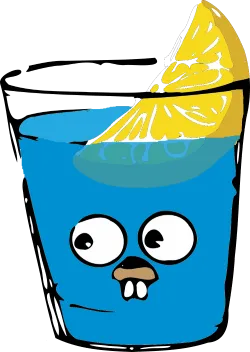
\includegraphics[width=40mm, keepaspectratio ]{pictures/gin.png}
  \caption[Poem]{รูปจาก https://www.askme.co.th/article/what-is-docker/}
  \label{fig:gin}
\end{figure}
\hspace{1.27cm}Gin\cite{Gin101} เป็น web framework ที่เขียนด้วยภาษา golang ที่ถูกพัฒนาต่อมาจาก Martini API ที่หยุดพัฒนาไปแล้ว โดย Gin จะใช้ customized httprouter ทำให้มีประสิทธิภาพด้านความเร็วที่สูงมากกว่า Martini ถึง 40 \cite{GinFeature}เท่า ทำให้มีperformance กับ productivity ที่ดี 

\subsubsection{Feature สำคัญของ Gin มีดังนี้ }
\begin{itemize}
  \item \textbf{JSON validation} สามารถแปลงและตรวจสอบ JSON ของ HTTP request
  \item \textbf{Routes grouping} จัดกลุ่ม routes ของ request ว่า request ไหนต้องมีการ authorization หรือไม่จำเป็นต้องมี การแยก request ด้วย version ของ API โดยสามารถจัดกลุ่มได้อย่างไม่จำกัด และไม่กระทบกับประสิทธิภาพ
  \item \textbf{Middleware support} incoming HTTP request จะถูกจัดการด้วย chain ของ middleware และ action สุดท้าย
  \item \textbf{Rendering build-in} ง่ายสำหรับสร้าง API ที่ render เป็น JSON, XML และ HTML
  \item \textbf{Error management} สามารถจัดการ error ที่เกิดขึ้นในระดับ application และ HTTP ได้
\end{itemize}

\section{RabbitMQ}
\hspace{1.27cm}RabbitMQ \cite{rabbitmq}ซอฟต์แวร์ที่เป็นตัวกลางรับส่งข้อความระหว่างแอปพลิเคชันต่างๆ ผู้ไปรับรับข้อความจากผู้ส่ง (แอปพลิเคชันหนึ่ง) เก็บไว้รอการคัดแยก และส่งต่อให้ผู้รับ (แอปพลิเคชันอีกแอปพลิเคชันหนึ่ง) เหมาะสำหรับการทำแอปพลิเคชันที่ต้องมีการจัดคิวในการส่งข้อความ ระบบที่เป็นไมโครเซอร์วิสเอาไว้สื่อสารกันได้อย่างมีประสิทธิภาพ ทำให้สามารถแบ่งงานขนาดใหญ่เป็นงานย่อยๆ และส่งไปยังระบบอื่นๆ เพื่อประมวลผลได้นั่นเอง
\begin{figure}[H] % 'H' forces placement exactly here
  % \begin{figure}[ht] % 'ht' means place it approximately here
    \centering
    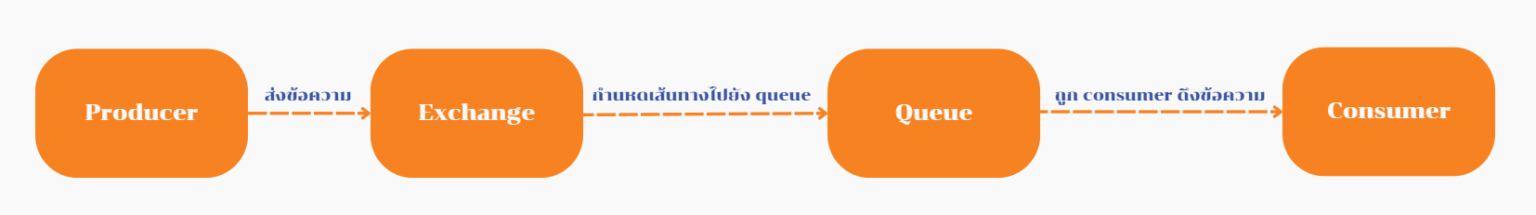
\includegraphics[width=\linewidth, keepaspectratio]{pictures/rabbitmq.png}
    \caption[Poem]{รูปจาก https://www.borntodev.com/2024/06/09/rabbitmq-nodejs/}
    \label{fig:rabbitmq}
\end{figure}
  \subsection{คำศัพท์ต่างๆที่เกี่ยวข้อง}
  \begin{itemize}
    \item \textbf{Producer} คือ ผู้ส่งข้อความ
    \item \textbf{Consumer} คือ ผู้รับข้อความ
    \item \textbf{Queue} คือ คิวข้อความ
    \item \textbf{Exchange} คือ ตัวกลางในการส่งข้อความ
    \item \textbf{Binding} คือ การเชื่อมต่อระหว่าง Exchange กับ Queue
    \item \textbf{Channel} คือ ช่องสื่อสารระหว่าง Producer และ Consumer
    \item \textbf{Connection} คือ การเชื่อมต่อระหว่าง RabbitMQ กับ Producer และ Consumer
  \end{itemize}
\subsection{Docker}
\begin{figure}[H]
  \centering
  
\includegraphics[width=100mm, keepaspectratio ]{pictures/docker.png}
  \caption[Poem]{รูปจาก https://www.docker.com/}
  \label{fig:docker}
\end{figure}

\hspace{1.27cm}Docker\cite{Docker}เป็นแพลตฟอร์มโอเพนซอร์สที่ช่วยในการสร้าง ทดสอบ และปรับใช้แอปพลิเคชันในรูปแบบของคอนเทนเนอร์ คอนเทนเนอร์เป็นสภาพแวดล้อมที่แยกจากกันที่สามารถรันแอปพลิเคชันได้ โดยที่ไม่ต้องกังวลเกี่ยวกับการกำหนดค่าหรือการติดตั้งซอฟต์แวร์เพิ่มเติมในระบบปฏิบัติการหลักของเซิร์ฟเวอร์ที่ใช้

\hspace{0.8cm}สิ่งที่ทำให้ Docker แตกต่างจากเทคโนโลยีอื่นๆ เช่น Virtual Machines (VMs) คือ Docker ใช้ Kernel ของระบบปฏิบัติการเดียวกันในการรันคอนเทนเนอร์แต่ละตัว ทำให้มีประสิทธิภาพในการใช้งานทรัพยากรสูงขึ้น และทำให้คอนเทนเนอร์ใช้เวลาในการเริ่มต้นที่รวดเร็ว

\subsection{องค์ประกอบหลักของ Docker}
\begin{itemize}
  \item \textbf{Docker Engine} เป็นซอฟต์แวร์ที่รันอยู่เบื้องหลังซึ่งทำหน้าที่สร้างและจัดการคอนเทนเนอร์ในระบบ มันมีองค์ประกอบย่อย 2 ส่วนที่สำคัญ ได้แก่
  \begin{enumerate}
    \item Docker Daemon (dockerd): เป็นโปรแกรมหลักที่รันอยู่เบื้องหลังและรับคำสั่งจาก Docker Client ผ่าน API โดย Daemon จะจัดการทุกอย่างที่เกี่ยวข้องกับคอนเทนเนอร์ เช่น การสร้าง, การเริ่มต้น, การหยุด, และการลบคอนเทนเนอร์
    \item Docker CLI (docker): คือส่วนที่ผู้ใช้ใช้ในการสั่งการ Docker ผ่านคำสั่งต่างๆ ผ่าน Command Line Interface เช่น การสร้างคอนเทนเนอร์ (docker run), การสร้างอิมเมจ (docker build), และการจัดการเครือข่าย (docker network)
  \end{enumerate}
  \item \textbf{Docker Image} คือไฟล์แบบคงที่ที่บรรจุโค้ดแอปพลิเคชันและทุกสิ่งที่แอปพลิเคชันนั้นต้องการในการรัน เช่น ไลบรารี, การตั้งค่า, และไฟล์ระบบ Image ถูกสร้างจากไฟล์ที่เรียกว่า Dockerfile ซึ่งเป็นไฟล์ที่กำหนดขั้นตอนในการติดตั้งและตั้งค่าแอปพลิเคชัน
  
  \textbf{Dockerfile Syntax} ที่ใช้ในการสร้าง Image มีคำสั่งที่เป็นลำดับขั้นตอน ยกตัวอย่างเช่น
  \hspace{1cm}\begin{enumerate}
    \item FROM: ระบุ Image เบื้องต้น เช่น Ubuntu, Alpine หรือ Node.js
    \item RUN: รันคำสั่งใน Image เช่น การติดตั้งแพ็คเกจ
    \item COPY/ADD: คัดลอกไฟล์จากโฮสต์เข้าสู่ Image
    \item CMD/ENTRYPOINT: กำหนดคำสั่งที่รันเมื่อคอนเทนเนอร์เริ่มทำงาน
  \end{enumerate}
  \item \textbf{Docker Container} คือ สิ่งที่ถูกสร้างจาก Docker Image และเป็นสภาพแวดล้อมที่แยกจากกันที่สามารถรันแอปพลิเคชันได้โดยมีคุณสมบัติดังนี้
  \item \begin{enumerate}
    \item แยกการทำงานจากระบบปฏิบัติการโฮสต์ แต่ยังใช้เคอร์เนลร่วมกัน
    \item สามารถสร้าง, ลบ, หยุด, และรีสตาร์ทได้อย่างง่ายดาย
    \item สามารถแชร์ทรัพยากรเครือข่ายและไฟล์ระหว่างคอนเทนเนอร์ต่างๆ ได้
  \end{enumerate}
\end{itemize}

\subsubsection{ความแตกต่างระหว่าง Docker กับ Virtual Machines}
\tolerance= 9999
\begin{table}[H]
  \centering
  \caption{เปรียบเทียบคุณสมบัติของ Docker และ Virtual Machine (VM)}
  \label{tab:docker-vm}

  \renewcommand{\arraystretch}{1.3} % Adjust row spacing
  \setlength{\extrarowheight}{3pt}  % Extra row height for better spacing
  \setlength{\tabcolsep}{8pt}       % Adjust column padding

  
  \begin{tabular}{|>{\raggedright\arraybackslash}p{3cm}|>{\raggedright\arraybackslash}p{5cm}|>{\raggedright\arraybackslash}p{5cm}|}
    % Balanced column widths
      \hline
      \rowcolor{gray!20} 
      \textbf{คุณสมบัติ} & \textbf{Docker} & \textbf{Virtual Machine (VM)} \\
      \hline
      การใช้เคอร์เนล & ใช้เคอร์เนลของระบบปฏิบัติการโฮสต์ & จำลองระบบปฏิบัติการเต็มรูปแบบ \\
      \hline
      ขนาดไฟล์ & ขนาดเล็ก & ขนาดใหญ่ \\
      \hline
      เวลาเริ่มต้น & เริ่มต้นได้อย่างรวดเร็ว & ใช้เวลามากขึ้น \\
      \hline
      การใช้ทรัพยากร & ใช้ทรัพยากรน้อย & ใช้ทรัพยากรมาก \\
      \hline
      ความยืดหยุ่น & เหมาะสำหรับแอปพลิเคชันแบบไมโครเซอร์วิส & เหมาะสำหรับการจำลองระบบขนาดใหญ่ \\
      \hline
      การแยกทรัพยากร & แยกการทำงานในระดับแอปพลิเคชัน & แยกระบบปฏิบัติการทั้งหมด \\
      \hline
  \end{tabular}
\end{table}

\hspace{1.27cm}โดยรวมแล้ว Docker เหมาะสำหรับการรันแอปพลิเคชันที่ต้องการความยืดหยุ่นในการปรับใช้และทรัพยากรที่มีข้อจำกัด ในขณะที่ VM เหมาะกับการรันระบบที่ต้องการการแยกสภาพแวดล้อมอย่างสมบูรณ์ เช่น การรันหลายระบบปฏิบัติการในเครื่องเดียวกัน

% \subsection{\ifenglish Hardware technology\else เทคโนโลยีด้านฮาร์ดแวร์\fi}
\section{Nginx Proxy Manager (NPM)}
\begin{figure}[H]
  \centering
  
\includegraphics[width=100mm, keepaspectratio ]{pictures/npm.png}
  \caption[Poem]{https://sparwan.com/en/blogs/news/tutoriel-installation-de-nginx-proxy-manager}
\end{figure}
\hspace{1.27cm}เป็น open-source ที่ออกแบบมาเพื่อช่วยให้การจัดการพร็อกซีของ Nginx, SSL ,Access Lists และอื่นๆ โดยสร้างขึ้นมาเพื่อจุดประสงค์ให้ง่ายต่อการใช้งานโดยมี Dashboard ให้ เหมาะสำหรับผู้ใช้ที่ไม่เชี่ยวชาญการใช้ Nginx ผ่าน CLI นอกจากนี้ ยังรองรับ SSL ฟรีผ่าน Let's Encrypt รวมถึงสามารถใช้งานได้บน Docker และรองรับการใช้งานหลาย User อีกด้วย
% \subsection{\ifenglish Software technology\else เทคโนโลยีด้านซอฟต์แวร์\fi}

\section{\ifenglish Project plan\else แผนการดำเนินงาน\fi}

\begin{plan}{6}{2020}{2}{2021}
    \planitem{7}{2020}{8}{2020}{ศึกษาค้นคว้า}
    \planitem{8}{2020}{1}{2021}{ชิล}
    \planitem{2}{2021}{2}{2021}{เผา}
    \planitem{12}{2019}{1}{2022}{ทดสอบ}
\end{plan}

\section{\ifenglish Roles and responsibilities\else บทบาทและความรับผิดชอบ\fi}
อธิบายว่าในการทำงาน นศ. มีการกำหนดบทบาทและแบ่งหน้าที่งานอย่างไรในการทำงาน จำเป็นต้องใช้ความรู้ใดในการทำงานบ้าง

\section{\ifenglish%
Impacts of this project on society, health, safety, legal, and cultural issues
\else%
ผลกระทบด้านสังคม สุขภาพ ความปลอดภัย กฎหมาย และวัฒนธรรม
\fi}

แนวทางและโยชน์ในการประยุกต์ใช้งานโครงงานกับงานในด้านอื่นๆ รวมถึงผลกระทบในด้านสังคมและสิ่งแวดล้อมจากการใช้ความรู้ทางวิศวกรรมที่ได้
